\chapter{Hiện thực hệ thống}
% \section{Công nghệ sử dụng}
% Để hiện thực hệ thống, nhóm quyết định sử dụng các công nghệ sau:
% \begin{itemize}
%     \item ReactJS: Hiện thực UI, frontend.
%     \item Java Springboot: Hiện thực microservice, backend.
%     \item PostgresSQL: Hệ cơ sở dữ liệu lưu trữ thông tin.
%     \item Kubernetes: Deploy các microservice.
%     \item Minikube: Chạy Kubernetes cluster trên local.
%     \item Terraform: Khởi tạo 
% \end{itemize}

% \section{Giới hạn phạm vi}
% \subsection{Về mặt nghiệp vụ}
% \noindent Sau khi bàn bạc, nhóm đi tới thống nhất là sẽ hiện thực phần Trang chủ (Home page - Catalog), vì đó là thành phần mà người dùng sẽ gặp đầu tiên khi bắt đầu truy cập vào hệ thống.
% \subsection{Về mặt thành phần hệ thống}
% \noindent Sau khi cân nhắc kỹ lưỡng, để đảm bảo cho phiên bản demo thể hiện được trọn vẹn và đầy đủ nhất các tính chất cốt lõi của hệ thống, nhóm đã giới hạn phạm vi hiện thực của hệ thống xuống còn các thành phần như sau:
% \begin{itemize}
%     \item Frontend: Trang chủ - Catalog, thể hiện danh sách các mặt hàng đang được bày bán 
%     \item Backend: Catalog service, cung cấp API danh sách sản phẩm.
%     \item Minikube cluster: Cung cấp môi trường Kubernetes cluster local trên máy tính cá nhân.
%     \item Deployment: Thành phần cơ bản nhất của hệ thống, dùng để quản lý trực tiếp các pod.
%     \item Service: Một lớp ảo hóa để các thành phần khác có thể truy cập tới các pod.
%     \item Ingress: Đóng vai trò như reverse proxy, cung cấp API gateway để kết nối từ bên ngoài cluster tới service.
%     \item Horizontal Pod Autoscaler: Dùng để tăng hoặc giảm số pod một cách tự động, dựa trên các thông số (metrics) của chính các pod đó.
% \end{itemize}
\section{Lựa chọn công nghệ và thư viện}
\section{Mã nguồn}
\subsection{Quản lý mã nguồn}
\noindent Git là một hệ thống quản lý phiên bản mã nguồn mở rất phổ biến, được sử dụng để quản lý mã nguồn trong các dự án phần mềm. Nó được Linus Torvalds phát triển vào năm 2005 và đã trở thành một công cụ không thể thiếu trong cộng đồng phần mềm mã nguồn mở. Git giúp các nhà phát triển dễ dàng và hiệu quả làm việc trên các phiên bản khác nhau của cùng một dự án, từ đó hỗ trợ quản lý và giám sát quá trình phát triển phần mềm. \\[0.5cm]
Nhóm đã lựa chọn \textbf{GitHub} để quản lý mã nguồn. GitHub là một dịch vụ lưu trữ mã nguồn trực tuyến (source code repository) và nền tảng hợp tác phát triển phần mềm dựa trên Git. GitHub cho phép các nhà phát triển lưu trữ, quản lý và chia sẻ mã nguồn của các dự án phần mềm.\\[0.5cm]
Ngoài ra, để việc đóng góp của các thành viên được diễn ra một cách bài bản và khoa học, nhóm đã định ra một bộ quy tắc về cách đặt tên branch, cách tạo, duyệt, gộp nội dung từ pull request vào branch chính, sẽ được trình bày cụ thể hơn ở phần phụ lục.

\subsection{Cấu trúc mã nguồn}
\noindent Nhóm đã tận dụng Github để quản lý mã nguồn cho 2 nội dung quan trọng nhất của đồ án, là báo cáo (được viết bằng Latex) và hệ thống, tương ứng với 2 repository. Mỗi repository đều có README ghi chú đầy đủ các nội dung hướng dẫn, giúp mỗi thành viên có thể nắm được các thông tin cơ bản của repository, đồng thời thực hiện các bước thiết lập nếu cần, trước khi có thể đóng góp nội dung vào đó.
\subsubsection{Mã nguồn báo cáo}
\noindent Do nội dung báo cáo không ít, do đó nhóm không ghi hết toàn bộ nội dung vào 1 file tex duy nhất, mà được chia ra thành nhiều file với cấu trúc như hình \ref{fig:thesis_source_code_structure}:
\begin{itemize}
    \item Thư mục \textbf{images}: Chứa toàn bộ các hình ảnh được sử dụng cho báo cáo. Bên trong còn được chia ra thành nhiều thư mục con, ứng với từng thành viên. Mỗi thành viên sẽ tự quản lý những hỉnh ảnh mà mình sử dụng trong báo cáo.
    \item Thư mục \textbf{sections}: Chứa nội dung của các chương trong báo cáo. Mỗi chương sẽ là 1 file tex riêng.
    \item File \textbf{main.tex}: Là khung xương của toàn bộ báo cáo, chứa các thiết lập, đồng thời là điểm bắt đầu để latex có thể biên tập nội dung.
    \item File \textbf{README.md}: Chứa đựng các thông tin cần thiết về repository. 
\end{itemize}
\begin{figure}[H]
    \begin{center}
        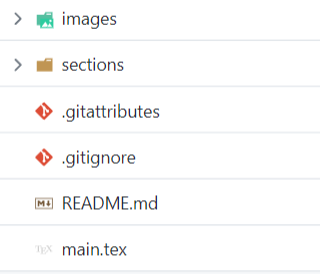
\includegraphics[scale = 1.5]{images/hanh/thesis-source-code-screenshot.png}
        \vspace*{2mm}
    \end{center}
    \caption{Cấu trúc mã nguồn của báo cáo}
    \label{fig:thesis_source_code_structure}

\end{figure}
\subsubsection{Mã nguồn hệ thống}
\section{Giao diện hệ thống}